\documentclass[tikz,border=3pt]{standalone}
\usepackage[utf8]{inputenc}
\usepackage[T1]{fontenc}
\usepackage{lmodern}
\renewcommand{\familydefault}{\sfdefault}
\usepackage{sansmath}\sansmath
\usepackage{chemfig}
\usepackage{pgfplots}\pgfplotsset{compat=1.18,/pgf/number format/use comma,/pgf/number format/1000 sep={.}}
\usetikzlibrary{arrows.meta,calc,positioning,decorations.pathmorphing,patterns}
% paleta del sitio
\definecolor{nar}{HTML}{E8680C}\definecolor{narc}{HTML}{FFB35C}\definecolor{hielo}{HTML}{FFF3E8}
\definecolor{tinta}{HTML}{1D1D1F}\definecolor{gris}{HTML}{6E6E73}\definecolor{lila}{HTML}{7C5CF0}
\definecolor{azul}{HTML}{2F6FD6}\definecolor{menta}{HTML}{17A673}\definecolor{coral}{HTML}{E8342A}
\begin{document}
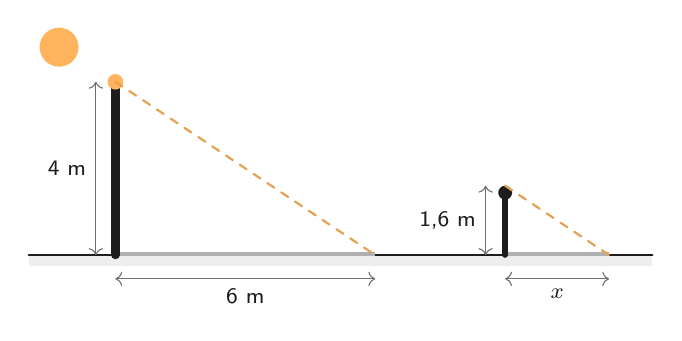
\begin{tikzpicture}[font=\small,x=0.55cm,y=0.55cm,line cap=round,line join=round,step={(1,1)}]
\fill[gris!12] (-2,-0.25) rectangle (12.4,0);
\draw[tinta,thick] (-2,0)--(12.4,0);
\fill[tinta!35] (0,-0.03) rectangle (6,0.08);
\draw[tinta,line width=3pt] (0,0)--(0,4);\fill[narc] (0,4) circle (0.18);
\draw[narc!90!black,thick,dashed] (0,4)--(6,0);
\draw[<->,gris] (-0.45,0)--(-0.45,4) node[midway,left,font=\footnotesize,text=tinta] {4 m};
\draw[<->,gris] (0,-0.55)--(6,-0.55) node[midway,below,font=\footnotesize,text=tinta] {6 m};
\fill[tinta!35] (9,-0.03) rectangle (11.4,0.08);
\draw[tinta,line width=2pt] (9,0)--(9,1.2800000000000002);\fill[tinta] (9,1.4400000000000002) circle (0.16000000000000003);
\draw[narc!90!black,thick,dashed] (9,1.6)--(11.4,0);
\draw[<->,gris] (8.55,0)--(8.55,1.6) node[midway,left,font=\footnotesize,text=tinta] {1,6 m};
\draw[<->,gris] (9,-0.55)--(11.4,-0.55) node[midway,below,font=\footnotesize,text=tinta] {$x$};
\fill[narc] (-1.3,4.8) circle (0.45);
\end{tikzpicture}
\end{document}
